\section{IRR-Filters}
\textbf{Infinite Impulse Response} filters where the impulse response of the system is of infinite duration.
\subsection{Design of IRR-filters}
Design of IRR-filters is done in the following steps:
\begin{enumerate}
  \item The specifications of the IRR-filter.
  \item The transfer function of the IRR-filter.
  \item The optimal realization of the IRR-filter.
  \item Program for signalprocessing or a circuit diagram for analog
    signalprocessing.
\end{enumerate}
\subsection{Matched z-transform}
By using the matched z-transform, the poles and zeros of the IRR-filter are directly transferred to the z-plane. The transfer function of the IRR-filter is given by:
$$z=e^{sT}$$

Following procedure is used for the matched z-transform:
\begin{enumerate}
  \item Determine the frequency-normalized and factorized transfer function $H(s)$ of the analog prototype filter.
  \item Determine the analog frequency-normalized poles and zero points.
  \item Determine the denormalized poles and zero points.
  \item Determine the coefficients of the digital transfer function.
  \item Implement the transfer function as a cascade structure.
\end{enumerate}
\subsubsection{1. Order Matched z-transformation}
The transfer function for a first order system is given by:
$$H(s)={\frac{s+A_{0}}{s+B_{0}}}={\frac{s-\sigma_{1}}{s-\sigma_{2}}}$$
where $-A_{0}=\sigma_1$ is a real zero and $-B_{0}=\sigma_2$ is a real pole of the IRR-filter.

A digital first order transfer function is given by:
$$H(z)={\frac{z-e^{\sigma_1 T}}{z-e^{\sigma_2 T}}}=\frac{1-e^{\sigma_1 T}z^{-1}}{1-e^{\sigma_2 T}z^{-1}}$$

A first order system without a zero is given by:
$$H(s)=\frac{\omega_a}{s+\omega_a}$$
Using the matched z-transform, the digital transfer function is given by:
$$H(z)=\frac{1}{1-e^{\sigma_1 T}z^{-1}}$$
where $\sigma_1$ is the pole of $H(s)$ and $T$ is the sampling period.\\
The transfer function $H(z)$ does not have a DC-gain of 1. To get a DC-gain of 1, the transfer function is multiplied by a gain factor $a_0$:
$$H(z)=\frac{a_0}{1+b_1z^{-1}}$$
where
$$b_0=-e^{\sigma_1 T} \qquad a_0=1+b_1$$
The corresponding digital realization structure:
\begin{center}
  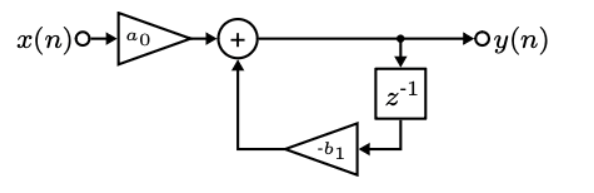
\includegraphics[width=0.4\textwidth]{Images/Matched-z-1th.png}
\end{center}
\subsubsection{2. Order Matched z-transformation}
The transfer function for a second order system with complex conjugate pole and zero pair is given by:
$$H(s)={\frac{s^{2}+A_{1}s+A_{0}}{s^{2}+B_{1}s+B_{0}}}$$
which has zeros in $s_1=\sigma_1+j\omega_1,s_1^*=\sigma_1-j\omega_1$ and poles in $s_2=\sigma_2+j\omega_2,s_2^*=\sigma_2-j\omega_2$

Using the matched z-transform:
$$H(z)={\frac{(z-e^{\sigma_{1}T}e^{j\omega_{1}T})(z-e^{\sigma_{2}T}e^{-j\omega_{1}T})}{(z-e^{\sigma_{2}T}e^{j\omega_{2}T})(z-e^{\sigma_{2}T}e^{-j\omega_{2}T})}}$$
Using Euler's identity:
$$H(z)=\frac{z^{2}-(2e^{\sigma_{1}T}\cos(\omega_{1}T))z+e^{2\sigma_{1}T}}{z^{2}-(2e^{\sigma_{2}T}\cos(\omega_{2}T))z+e^{2\sigma_{2}T}}=\frac{1-(2e^{\sigma_{1}T}\cos(\omega_{1}T))z^{-1}+e^{2\sigma_{1}T}z^{-2}}{1-(2e^{\sigma_{2}T}\cos(\omega_{2}T))z^{-1}+e^{2\sigma_{2}T}z^{-2}}$$
A second order low-pass filter is given by:
$$H(z)=\frac{a_0}{1+b_1z^{-1}+b_2z^{-2}}$$
where
$$a_0=1+b_1+b_2 \qquad b_1=-2e^{\sigma_1 T}\cos(\omega_1 T) \qquad b_2=e^{2\sigma_2 T}$$
The corresponding digital realization structure:
\begin{center}
  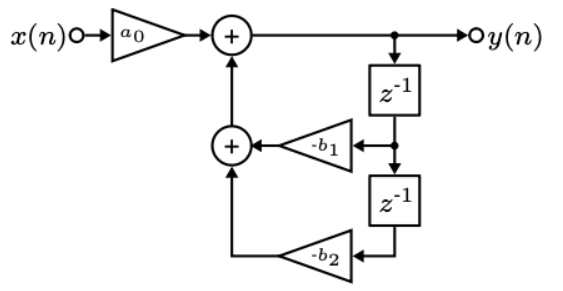
\includegraphics[width=0.4\textwidth]{Images/Matched-z-2nd.png}
\end{center}
\subsection{Impulse invariance method}
The following procedure is used to design digital IIR filters using the impulse invariant z transform.
\begin{enumerate}
  \item Determine the frequency-normalized transfer function $H(s)$ of the analog prototype filter.
  \item Partial fractionally resolve $H(s)$ into 1st and 2nd order transfer functions (maximum number of 2nd order transfer functions).
  \item Denormalize the coefficients $k_i$ and the poles $\sigma_i+j\omega_i$ by multiplication with the cutoff frequency or center frequency.
  \item Determine the coefficients of the digital transfer function.
  \item Implement the transfer function as a parallel structure.
\end{enumerate}

To find impulse invariant z-transformation, the impulse response is z-transformed:
$$H(z)=T\cdot \mathcal{Z}[h(n)]$$
Given a N'th order filter:
$$H(s)=\frac{\sum_{i=0}^M A_is^i}{\sum_{i=0}^N B_is^i}\qquad M\leq N$$
where $s_i$ is the i pole of the analog filter.

Using partial fractions, it can be written as:
$$H(s)=\sum_{i=1}^N \frac{k_i}{s-s_i}$$
And the z-transformation is:
$$H(z)=T\cdot \sum_{i=1}^N \frac{k_i}{1-e^{s_i T}z^{-1}}$$

\subsection{1st Order System}
$$H(s)=\frac{A_0}{s+B_0}=\frac{-\sigma_i}{s-\sigma_i}$$
Using the impulse invariant z-transformation:
$$H(z)=\frac{a_0}{1+b_1z^{-1}}$$
where
$$a_0=-\sigma_i T \qquad b_1=-e^{\sigma_iT}$$
\subsection{2nd Order System}
$$H(s)=\frac{A_0}{s^2+B_1s+B_0}$$
Find the partial fractions:
$$H(s)=\frac{k_i}{s-s_i}+\frac{k_i^*}{s-s_i^*}$$
where
$$s_i=\sigma_i+j\omega_i\qquad k_i=\alpha_i+j\beta_i$$
Using the impulse invariant z-transformation:
$$H(z)=\frac{a_0+a_1z^{-1}}{1+b_1z^{-1}+b_2z^{-2}}$$
where
$$a_0=-2\alpha_i T \qquad a_1=-2e^{\sigma_iT}(\alpha_i\cos(\omega_iT)-\beta_i\sin(\omega_iT))$$
$$b_1=-(2e^{\sigma_iT}\cos(\omega_iT)) \qquad b_2=e^{2\sigma_iT}$$

\subsection{Bilinear z transformation}
The following is the procedure for the design of digital filters using bilinearz transformation.
\begin{enumerate}
  \item The prewarping constant is determined as
    $$C=\cot\left(\frac{\omega_iT}{2}\right)$$
    where $i=a$ for low pass or high pass filter design and $i=c$ for band pass or band stop filter design.
  \item The order number of the filter is determined based on the prewarped stopband frequency.
  \item The frequency-normalized and factorized analog transfer functionH(s)is set up.
  \item The coefficients of the digital transfer function are calculated.
  \item The filter is implemented as a cascaded realization structure.
\end{enumerate}
\subsubsection{Warping and Pre-warping}
$$\Omega={\frac{2}{T}}\tan\left({\frac{\omega T}{2}}\right)\qquad\mathrm{\left[rad/s\right]}$$
$$\omega={\frac{2}{T}}\tan^{-1}\left({\frac{\Omega T}{2}}\right)\qquad\mathrm{\left[rad/s\right]}$$

$$\Omega_a=C\tan\left({\frac{\omega_a T}{2}}\right)\qquad\mathrm{\left[rad/s\right]}$$
Normalized stop-band frequency:
$$\frac{\Omega_i}{\Omega_s}=\frac{1}{\Omega_s}$$
where $i=a$ for low and high pass and $i=c$ for band-pass and band-stop.
\subsubsection{1st Order Bilinear z transformation}
First order system:
$$H(s)=\frac{A_{1}s+A_{0}}{B_{1}s+B_{0}}$$
Using bilinear z transformation:
$$H(z)=\frac{a_0+a_1z^{-1}}{1+b_1z^{-1}}$$
where
$$a_{0}=\frac{A_{0}+A_{1}C}{B_{0}+B_{1}C}\qquad a_{1}=\frac{A_{0}-A_{1}C}{B_{0}+B_{1}C}\qquad b_{1}=\frac{B_{0}-B_{1}C}{B_{0}+B_{1}C}$$
\subsubsection{2nd Order Bilinear z transformation}
A second order system:
$$H(s)={\frac{A_{2}s^{2}+A_{1}s+A_{0}}{B_{2}s^{2}+B_{1}s+B_{0}}}$$
Using bilinear z transformation:
$$H(z)={\frac{a_{0}+a_{1}z^{-1}+a_{2}z^{-2}}{1+b_{1}z^{-1}+b_{2}z^{-2}}}$$
where
$$a_{0}=\frac{A_{0}+A_{1}C+A_{2}C^{2}}{B_{0}+B_{0}C+B_{2}C^{2}}\qquad a_{1}=\frac{2(A_{0}-A_{2}C^{2})}{B_{0}+B_{1}C+B_{2}C^{2}}\qquad a_{2}=\frac{A_{0}-A_{1}C+A_{2}C^{2}}{B_{0}+B_{1}C+B_{2}C^{2}}$$
$$b_{1}=\frac{2(B_{0}-B_{2}C^{2})}{B_{0}+B_{1}C+B_{2}C^{2}}\qquad b_{2}=\frac{B_{0}-B_{1}C+B_{2}C^{2}}{B_{0}+B_{1}C+B_{2}C^{2}}$$
\subsection{Examples}
\subsubsection{Example 1: Matched 1st order z-transform}
Consider the following analog first order lowpass filter with cutoff frequency $\omega_a=2\pi f_a$ where $f_a=\SI{300}{\hertz}$:
$$H(s)=\frac{\omega_a}{s+\omega_a}=\frac{1885}{s+1885}$$
which has a pole in $s_1=\sigma_1=-1885$.\\
Find the digital IRR-filter using the matched z-transform with sampling frequency $f_s=\SI{16}{\kilo\hertz}$.

\rule{\textwidth}{0.5pt}

The coefficients of the digital IRR-filter are given by:
$$b_1=-e^{\sigma_1 T}=-e^{-1885\cdot\frac{1}{16000}}=-0.8889$$
$$a_0=1+b_1=0.1111$$
The digital lowpass filter is given by:
$$H(z)=\frac{a_1}{1+b_0z^{-1}}=\frac{0.1111}{1-0.8888z^{-1}}$$

\subsubsection{Example 2: Matched 3rd order matched z-transform}
Consider the following Butterworth 3rd order low-pass filter (frequency-normalized filter) 
and design an equivalent digital low-pass filter with cut-off frequency at $\SI{1}{\kilo\hertz}$ and sample frequency at $\SI{8}{\kilo\hertz}$. 
$${\tilde{H}}(s)=\frac{1}{s+1}\frac{1}{s^{2}+s+1}$$
Using the matched z-transform

\rule{\textwidth}{0.5pt}

\textbf{1. Determine the frequency-normalized and factorized transfer function $H(s)$ of the analog prototype filter.}\\
Is in this case it's already given.

\textbf{2. Determine the analog frequency-normalized poles and zero points.}\\
There is no zeros in the transfer function, so only the poles are determined:
$$s_1=-1 \qquad s_2=s_2^*=-\frac{1}{2}+j\frac{\sqrt{3}}{2}$$

\textbf{3. Determine the denormalized poles and zero points.}\\
Only the poles are denormalized, since there are no zeros:
$$\omega_a=2\pi f_a=2\pi\cdot 1000=6283.2$$
$$\sigma_1=-1\cdot\omega_a=-6283.2$$
$$\sigma_2\pm j\omega_2=s_2\cdot\omega_a=-3141.6\pm j5434.4$$

\textbf{4. Determine the coefficients of the digital transfer function.}
$$H(s)=H_1(s)H_2(s)=\frac{1}{s+1}\frac{1}{s^{2}+s+1}$$
$$H(z)=H_1(z)H_2(z)$$
Using the matched z-transform:
$$H_1(z)=\frac{1}{1-e^{\sigma_1 T}z^{-1}}=\frac{a_{0_1}}{1+b_{1_1}z^{-1}}$$
$$b_{1_1}=-e^{\sigma_1 T}=-e^{-6283.2\cdot\frac{1}{8000}}=-0.4559\qquad a_{0_1}=1+b_{1_1}=0.5441$$
$$H_1(z)=\frac{0.5441}{1-0.4559z^{-1}}$$
and
$$H_2(z)={\frac{1}{(z-e^{\sigma_{2}T}e^{j\omega_{2}T})(z-e^{\sigma_{2}T}e^{-j\omega_{2}T})}}=\frac{a_{0_2}}{1+b_{1_2}z^{-1}+b_{2_2}z^{-2}}$$
$$b_{1_2}=-2e^{\sigma_2 T}\cos(\omega_2 T)=-2e^{-3141.6\cdot\frac{1}{8000}}\cos(5434.4\cdot\tfrac{1}{8000})=-1.0507$$
$$b_{2_2}=e^{2\sigma_2 T}=e^{2\cdot -3141.6\cdot\frac{1}{8000}}=0.4559$$
$$a_{0_2}=1+b_{1_2}+b_{2_2}=1-1.0507+0.4559=0.4052$$
$$H_2(z)=\frac{0.4559}{1-1.0507z^{-1}+0.4559z^{-2}}$$

Combining the two transfer functions:
$$H(z)=H_1(z)H_2(z)=\frac{0.5441}{1-0.4559z^{-1}}\frac{0.4052}{1-1.0507z^{-1}+0.4559z^{-2}}$$

\subsubsection{Example 3: Matched 3. order impulse invariance z-transform}
Consider the following Butterworth 3rd order low-pass filter (frequency-normalized filter) 
and design an equivalent digital low-pass filter with cut-off frequency at $\SI{1}{\kilo\hertz}$ and sample frequency at $\SI{8}{\kilo\hertz}$. 
$${\tilde{H}}(s)=\frac{1}{s+1}\frac{1}{s^{2}+s+1}$$
Using the impulse invariance method

\rule{\textwidth}{0.5pt}

\textbf{1. Determine the frequency-normalized and factorized transfer function $H(s)$ of the analog prototype filter.}\\
Is in this case it's already given.

\textbf{2. Partial fractionally resolve $H(s)$ into 1st and 2nd order transfer functions (maximum number of 2nd order transfer functions).}\\
The poles are given by:
$$s_1=-1 \qquad s_2=s_2^*=-\frac{1}{2}+j\frac{\sqrt{3}}{2}$$
The transfer function is given by:
$$H(s)=\frac{k_1}{s-(s_1)}+\frac{k_2}{s-(s_2)}+\frac{k_2^*}{s-(s_2^*)}=\frac{k_1}{s-(-1)}+\frac{k_2}{s-(-\frac{1}{2}+j\frac{\sqrt{3}}{2})}+\frac{k_2^*}{s-(-\frac{1}{2}-j\frac{\sqrt{3}}{2})}$$


\textbf{3. Denormalize $k_i$ and the poles}

\textbf{4. Find the coefficients of the digital transfer function}
\subsubsection{Example 4: Bilinear z-transform}
An analog 5th order Butterworth low-pass filter $H(s)$ has a -3 dB cut-off frequency $f_3= 3$ kHz and -30 dB stopband frequency $f_{30}= 6$ kHz. 
The filter is digitized by bilinear z-transformation with a sample rate of 16 kHz. 

\rule{\textwidth}{0.5pt}

$$N\left[\frac{2 \tan ^{-1}\left(\frac{3000\ 2 \pi }{16000\ 2}\right)}{\frac{1}{16000}}\right]$$
